% \documentclass[twocolumn]{article}
\documentclass[12pt]{article}
\usepackage[utf8]{inputenc}
\usepackage{natbib}
\usepackage{graphicx, caption}
\usepackage{authblk}
\usepackage{textcomp}
\usepackage[usenames,dvipsnames]{xcolor}
\usepackage{amsmath}
\usepackage{cuted}

\usepackage{multicol}
\usepackage[textwidth=492.982pt, top=2cm, bottom=2cm]{geometry}

\usepackage{setspace}
\doublespacing

\graphicspath{{./figures}{./}}

\title{Chapter 16: Particle-laden gravity currents: the lock-release slumping regime at the laboratory scale}

% \title{Chapter 16: Lock-release particle-laden gravity currents at the laboratory scale}

% \title{Macroscopic description of particle-laden gravity currents: overall perspectives}

% \title{Macroscopic description of lock-release particle-laden gravity currents}

\author[1]{Gadal C.}
\author[2]{Schneider J.}
\author[3]{Bonamy C.}
\author[3]{Chauchat J.}
\author[2]{Dossmann Y.}
\author[2]{Kiesgen de Richter S.}
\author[1]{Mercier M. J.}
\author[4]{Naaim-Bouvet F.}
\author[3]{Rastello M.}
\author[1]{Lacaze L.}

\affil[1]{Institut de Mécanique des Fluides de Toulouse (IMFT), Université de Toulouse, CNRS, Toulouse, France}
\affil[2]{Laboratoire Énergies et Mécanique Théorique
et Appliquée (LEMTA), Université de Lorraine, CNRS, 54500, Nancy, France}
\affil[3]{Univ. Grenoble Alpes, CNRS, Grenoble INP, LEGI, 38000 Grenoble, France}
\affil[4]{Univ. Grenoble Alpes, INRAE, CNRS, IRD, Grenoble INP, IGE, 38000 Grenoble, France}


\begin{document}

\maketitle

\begin{abstract}

	Particle-laden gravity currents (PLGCs) are driven by the mass difference between a heavy fluid-particle mixture and a lighter ambient liquid. They often occur in natural and industrial situations, among which a typical situation is the release of a finite volume. Here, we focus on such `dam-break' situations, which are studied using lock-release devices at the laboratory scale.
	%
	The objective of the present chapter is to provide a description at the macroscopic scale of the early moments of the flow, namely the \emph{slumping regime}, with respect to the relevant dimensionless parameters. For this, we combine a total of 288 runs from three different lock-release devices and from two-fluids numerical simulations, which allow us to cover a large range of particle types (size and density), volume fractions, bottom slopes and geometries.
	%
	By tracking the front propagation through time, we extract the dimensionless slumping velocity $\mathcal{F}r$ and dimensionless characteristic slumping duration $\tau$, on which we base our description.
	%
	Our results show that the slumping velocity increases with the bottom slope, but decreases with the particle volume fraction when the latter exceeds a critical value. However, it remains independent of particle settling processes, which on the other hand affects the slumping duration. Hence, above a critical threshold, $\tau$ decreases as the ratio between the settling velocity and characteristic current velocity increases. For all these regimes, we derive scalings and energetic balances that reproduce the observed trends. The latter comparison confirms the role of initial energy transfer from the initial state towards the slumping phase on the resulting dynamics. This initial process and its characterisation remain crucial to prescribe relevant initial conditions for large-scale predictive modelling.

\end{abstract}


\section{Introduction}
\label{sec:intro}

\subsection{Finite volume density currents}
\label{sec:intro_lockrelease}

Density currents have been widely considered at the laboratory scale for their ubiquitous occurrence in geophysical flows \citep{Hopfinger1983,Simpson1999,Dufek2016}. As they are mostly associated with unsteady and non-uniform dynamics in nature, the lock-release device appeared to be a popular canonical configuration to mimic their behaviour at the laboratory scale \citep{Hacker1996,Shin2004,Nogueira2014}. In particular, studies often focused on characterising the front dynamics and the front shape as a macroscopic description of the underlying complex dynamics \citep{Rottman1983,Marino2005,Hogg2006}.

The basic approach to describe a lock-release evolution is built upon characteristics solutions of the hyperbolic shallow water equations for an inviscid dense liquid of density $\rho_{\text c}$ slumping on a horizontal bottom under an inertialess and weightless ambient fluid. In particular, this allows predicting the front velocity $U_{\text{c}}$ only based on the initial condition of the released mass. At the early stages of the slumping phase, it is found to be simply related to the only velocity scale of the system as
\begin{equation}
	U_{\text{c}}\propto \sqrt{gH_0},
\end{equation}
with $g$ gravitational acceleration and $H_0$ the initial height of the fluid volume being released. The method of characteristics suggests a coefficient of proportionality of exactly $2$ between velocities $U_{\text{c}}$ and $\sqrt{g H_0}$. An extension towards a weighted ambient fluid of density $\rho_{\text a}$ could lead to
\begin{equation}
	\label{eq:solUc}
	U_{\text{c}}=F\sqrt{\tilde{g}H_0},\quad\mbox{with}\quad \tilde{g}=\frac{\rho_{\text c}-\rho_{\text a}}{\rho_{\text c}}g,
\end{equation}
However, the coefficient of proportionality $F$, similar to a Froude number, now requires slightly more attention as it is clearly found smaller than $2$ in experiments or simulations. The main reason is that most density currents are characterized by a small density ratio between current and ambient, making the assumption of inertialess ambient fluid unlikely. A dynamic front condition is now required, and is often inspired from the steady front configuration derived by \citet{Benjamin1968}, now also linking the ambient height $H_{\text a}$ to the front velocity. This front relation includes two unknowns, a front velocity and a front height, and is often used as a front boundary condition in shallow water numerical solver for gravity currents \cite[e.g.][]{Ungarish2009}. Then, past studies managed to link the front velocity to the current height close to the front. However, the link between the front velocity and the initial conditions then becomes much more difficult to predict.
Models have been proposed to circumvent this issue, leading for instance to \citep{Huppert1980}
\begin{equation}
	\label{eq:Froude_Huppert1980}
	F = 0.5 \sqrt{\frac{\rho_{\text c}}{\rho_{\text a}}}\left(\frac{H_{\text a}}{H_0}\right)^{1/3}.
\end{equation}
%
The latter is relevant for not too deep ambient $H_{\text a}$ compared to the reservoir height $H_0$, which is actually the case in most experiments. Many configurations correspond to full-depth release ($H_{\text a}=H_0$), which leads to $F = 0.5(\rho_{\text c}/\rho_{\text a})^{1/2}$. Even if several experiments and numerical simulations confirm such a result, the exact value of $F$ remains still unclear and probably dependent on several physical processes. In particular, these relationships during the slumping regime are based on assuming negligible dissipation, which shall be violated in some cases, for instance in the presence of settling particles or significant mixing with the ambient at the miscible interface.

For a finite volume lock-release device on a mild enough slope, the slumping regime necessarily ends when the rarefaction wave associated with finite volume reaches the current front \citep[e.g.][]{Rottman1983, Hogg2006}. This leads to a new regime usually referred to as the inertial regime in the literature. This is observed on the front evolution as $U_{\text{c}}$ is no longer time independent but evolves as $t^{-1/3}$.
A simple approach can be useful to provide a rapid estimation of the position $X_{\text t}$ or time $T_{\text t}$ at which this transition occurs. For that purpose, it is worth mentioning that such a transition occurs as a rarefaction wave evolves faster than the front. Then, assuming the front velocity $U_{\text{c}}$ to be different from the rarefaction wave velocity at the interface $\sqrt{\tilde{g}H_0}$, which is assumed to be constant along its entire propagation path for simplicity, this leads to a transition length scale $X_{\text t}$ written as
\begin{equation}
	\label{eq:Xt_inertial}
	\displaystyle X_{\text t}\propto  \frac{2L_0 F}{1 - F}.
\end{equation}
Note that here $2$ comes from the path of propagation of the wave: emanating from the gate, it propagates backwards to the end of the reservoir, reflects on the wall and then propagates towards the front.
During the slumping regime, the previous estimation of $F$ \eqref{eq:Froude_Huppert1980} for full depth release $H_0=H_{\text a}$ leads to $X_{\text t}\propto 2L_0/[2(\rho_{\text a}/\rho_{\text c})^{1/2}-1]$. Note that, although more advanced methods based on single-layer shallow-water models predict a similar result, $X_{\text t} = 2 L_0 F (1 + F/2)^{1/2}$ \citep{Hogg2006}, full depth-release experiments have found much larger transitional positions, i.e $X_{\text t} \approx 10 L_{0}$~\citep{Rottman1983}.

Other mechanisms can modify the dynamics of the slumping regime which could lead to other transitions of the front velocity at different positions $X_{\text t}$ or times $T_{\text t}$, prior to the influence of the rarefaction wave. This is basically part of the topic of the present chapter.

For a gravity current on a horizontal bottom, a classic transition discussed in the literature is the one dominated by viscous dissipation. The flow eventually reaches a fully viscous regime \citep{Huppert1980}. This transition typically holds for fully laminar flow. A similar regime can be induced by inertial friction, for which the full derivation remains less obvious \citep[see for instance][for the case of a constant-influx current]{Hogg2001}. In any case, such transition can be seen as the time or position at which the current is strongly affected by dissipation, which actually encompasses entrainment for miscible gravity currents. The slumping regime then ends when dissipation induced by bottom friction and/or entrainment at the miscible interface, overcomes the current dynamics.
%
Again using a simple idealised approach, the latter transition can be estimated from a dynamic condition balancing an estimation of the shear stress $\rho_{\text c} C_d U_{\text{c}}^2$ ($C_d$ being some drag coefficient induced by friction at the bottom and/or by entrainment at the interface) with inertia over the current height $h_{\text c}$, $\rho_{\text c} U_{\text{c}}^2 h_{\text c} /X_t$. In the latter expression, $h_{\text c}$ can have different scaling. In the case of a clearly detached current head, the constant height scales with the initial height $H_0$. When assuming that the current remains attached to the initial column at transition \citep[similarly to][but for inertial drag instead of viscous dissipation]{Bougouin2022}, mass conservation between the initial column and a simplified box geometry implies $h_{\text c} = H_0 L_0/X_t$.
%
Both cases respectively lead to
\begin{equation}
	\label{eq:Xt_drag}
	\displaystyle X_{\text t}= {\frac{H_0}{C_d}}\quad \mbox{or} \quad X_{\text t}=  \sqrt{\frac{H_0 L_0}{C_d}}.
\end{equation}

To finish with, constant bottom slope $\alpha$, often relevant to characterize the main process of natural flow over topography, adds complexity to this front analysis. First, note that, when considering an inclined bottom, the reduced gravity and therefore the characteristic velocity \eqref{eq:solUc} shall be updated with a $\cos{\alpha}$ term accounting for the reduced effect of the initial column pressure normal to the inclined bottom. Second, including a bottom slope also adds a constant forcing along the slope suggesting a constant acceleration of the flow, at least until balanced by friction at both the interface and the bottom. Hence, it could affect the existence of the aforementioned slumping constant-velocity regime.
%
Yet, constant velocities associated with a slumping regime are clearly observed at early stages in experiments and simulations prior to such balance \citep{Birman2007, Gadal2023}. This is due to the relatively long time or length scales required for slope-induced acceleration to overcome the flow induced by the initial pressure gradient. A way to highlight that is a simple balance between slope and pressure gradient, resulting in
\begin{equation}
	\label{eq:Xt_slope}
	X_{\text t}=H_0\tan^{-1}{(\alpha)}.
\end{equation}
The latter can be seen as a transition length scale after which the slope starts driving the current until reaching the next equilibrium between slope and friction.


%%%%%%Figure 1
\begin{figure*}[ht!]
	\centering
	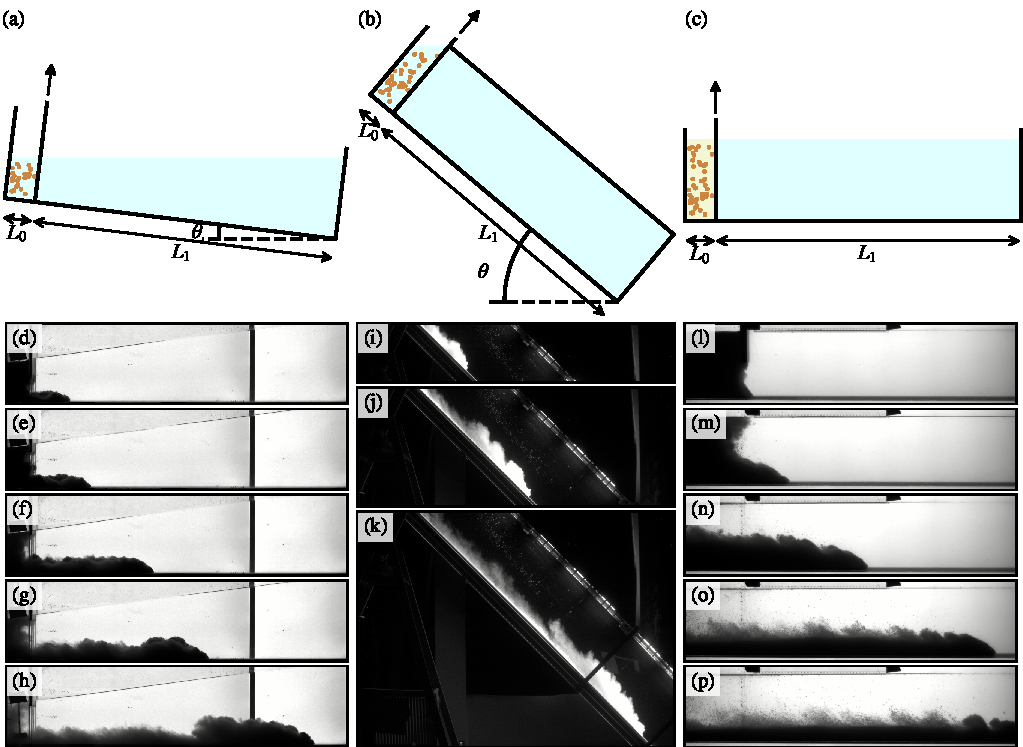
\includegraphics{figure1.pdf}
	\caption{\textbf{Experimental set-ups used in this study.} (a--c) Sketches of the three experimental set-ups. Below are shown snapshots of corresponding experimental images: (d--h) Set-up 1, $\alpha = 7^\circ$, $\phi \sim 3~\%$, ${S}t=0.027$; (i--k) Set-up 2, $\alpha = 45.4^\circ$, $\phi \sim 1.5~\%$, ${S}t=0.06 $; (l--p) Set-up 3, $\alpha = 0^\circ$, $\phi \sim 55\%$, ${S}t \equiv 0$; (q--v) SedFoam, $\alpha = 45.4^\circ$, $\phi \sim 1.7~\%$, $\mathcal{S}t=0.06$.}
	\label{fig:fig1}
\end{figure*}
%%%%%%%%


\subsection{Particle-Laden Gravity Currents}
\label{sec:intro_PLGC}

Particle-Laden Gravity Currents (PLGCs) refer to as gravity currents, or density currents, are driven by a mass difference between a heavy fluid-particle mixture and a lighter ambient liquid \citep[e.g.][]{Hopfinger1983,Middleton1993,Kneller2000,Meiburg2010,wells2021}. Different subclasses of PLGCs can be distinguished depending on the relative density of the different phases constituting the system; i.e. the particle phase, the carrier fluid phase and the ambient fluid phase. In the following, we will focus on two of them, characterized by only two distinct densities. At one end, the carrier phase and ambient phase are the same fluid and particles are heavier. This is the most commonly studied subclass of PLGCs, usually referred to as turbidity currents. At the other end, PLGCs can also be induced by a neutrally-buoyant fluid-particle mixture flowing into a lighter ambient fluid.

A major difference between PLGCs and compositional currents is therefore the existence of typical length and time scales associated with the particle dynamics. Nevertheless, the prediction of these finite scales is difficult as it shall strongly depend on the interaction between particle dynamics and the local turbulence of the carrying fluid and/or ambient fluid at the upper interface which modifies entrainment and associated dissipation. In turn, this can modify the macroscopic behaviour of the current, for instance, the dynamics of the front. Accordingly, these dynamics shall be controlled by several dimensionless parameters that can lead to a wide variety of flow regimes. In particular, beyond the slope $\alpha$, the dimensionless density difference between the current and the ambient $\mathcal{A}t$, the ratio between available inertia and dissipation, say a Reynolds number $\mathcal{R}e$ as usually introduced as a control parameter for any density currents, the initial solid fraction of particles $\phi$ and a dimensionless settling velocity $S=V_{\text s}/U_{\text{c}}$ with $V_{\text s}$ the settling velocity of particles into the carrying fluid phase, have now to be considered as potentially affecting flow regimes. It shall be noted that in some specific situations, some of these dimensionless parameters could be linked (for instance $\phi$ and $\mathcal{A}t$ for heavy particles in a single-phase liquid for the carrying and ambient fluids).

Beyond the transition from the slumping regime to other regimes discussed in the previous section (still relevant for PLGCs although parametrisation of the processes involves more complex mechanisms induced by the fluid-particle interaction), here, a new transition towards the deposition of the particle can emerge. In particular, based on a kinematic approach balancing time scales related to current propagation and particle settling, leads to
%
\begin{equation}
	\label{eq:Xt_settling}
	X_{\text t} \propto H_0\frac{U_{\text{c}}}{V_{\text s}}.
\end{equation}
%
Note that such transition shall disappear for the neutrally-buoyant situation of PLGCs.
However, it has been observed that mixing at the interface can modify the local concentration of particles at the front, resulting in behaviour similar to that of settling~\cite{Schneider2023}. Again, such an approach only gives a scaling of transition, but the influence of the particle dynamics prior to such transition remains unclear. Overall, the value of $F$ in \eqref{eq:solUc} during the slumping inertial regime remains to clarify varying the influence of the mechanisms discussed so far.

Even if the dynamics of PLGCs is associated with several complex processes, a general consequence is observed in the front dynamics, often referred to as the Froude number, and the front shape. Then prediction of the different flow regimes associated with PLGCs shall be somewhat included in these observables. After presenting the experimental and numerical methods used to investigate PLGCs dynamics in section~\ref{sec:methods}, we introduce the main dimensionless quantities used and macroscopic observations in section~\ref{sec:current_description}. We discuss our results in section~\ref{sec:results} and conclude in section~\ref{sec:conclusion}.

\section{Methods}
\label{sec:methods}

In order to characterize the slumping regime, and its transition to other regimes, of PLGCs induced by the finite-volume release of a suspension initially at ``rest'', 3 lock-release devices have been used to cover a wide range of control parameters. These experimental devices are supplemented with two-fluid numerical simulations to confirm the relevance of such a flow description to characterize the dynamics of PLGCs.

\subsection{Experimental set-ups}

All set-ups are based on the same typical lock-release design (see figure~\ref{fig:fig1}). The tank has a width $W$, a height $H$ and a length $L_0 + L_1$ along the $x$ direction. It is split into two parts by a sluice gate at a distance $L_0$ from the left wall. %More specifically, a tank of width $W$, height $H$ and length $L_0+L_1$ along the streamwise direction $x$ is split in two along this direction by a sluice gate at a distance $L_0$ from one end. 
On the $L_0$ side, a reservoir is filled up to a height $H_0$ with a fluid/particle mixture having a density $\rho_{\text{m}} = \phi \rho_{\text{p}} + (1 - \phi)\rho_{\text{f}}$, with $\rho_{\text{p}}$ and $\rho_{\text{f}}$ the particle and fluid densities, respectively. On the other side of height $H_{\text a}$ is the ambient fluid of density $\rho_{\text{a}}$, with typically $\rho_{\text{a}} < \rho_{\text{m}}$. At $t = 0$, the sluice gate is lifted up manually to initiate the gravity current.

\paragraph{Set-up 1}

The first set-up (figure~\ref{fig:fig1}(a)) has $L_0+L_1=150~{\text cm}$ with $L_0 = 10~\textrm{cm}$, $W = 10~\textrm{cm}$ and $H=49~\textrm{cm}$. The upper boundary is a free surface and the tank can be inclined at an angle $\alpha\in[0^\circ,7.5^\circ]$ with respect to the horizontal as shown in the 2D sketch of figure~\ref{fig:fig1}(a). For inclined configurations, $H_{\text a}$ then increases along the flume, and the reservoir is filled such as both heights at the gate, reservoir one and ambient one, are the same (see figure~\ref{fig:fig1}(a)). The suspension in the reservoir is made by strongly stirring a known mass of particles within the whole water column using a mechanical mixer, which is stopped just before opening the gate. $H_{0}$ is defined as the average suspension height inside the lock, equal to $20~\textrm{cm}$.
%
The current evolution is followed by an sCMOS pco.edge$^\copyright$ camera at 120 Hz, using a LED backlight as a light source. Additional details on the set-up and the image processing can be found in \citet{Gadal2023}.

\paragraph{Set-up 2}
The second set-up (figure~\ref{fig:fig1}(b)) has $L_0+L_1=3.8~{\text m}$ with $L_0 = 30~\textrm{cm}$ for runs with PMMA particles and $L_0 = 10~\textrm{cm}$ for runs with silica sand or hydrogel particles (see section~\ref{sec:datasets} for particles specifications). The overall flume width and depth are $W= 10~\textrm{cm}$ and $H= 50~\textrm{cm}$. The upper boundary in the flume is a rigid lid, and the only free surface is in the lock region. The ambient fluid is tap water at room temperature and $H_{\text a}=50~\textrm{cm}$. The flume can be inclined at an angle $\alpha \in [0^\circ,45.4^\circ]$ as shown in figure~\ref{fig:fig1}(b). Here, $H_0$ is defined as the average suspension depth perpendicular to the flume floor inside the lock at the gate opening time. LED plates illuminate the flume from above. The flow dynamic is recorded with a Phantom$^\copyright$ Miro C110 camera at 50 Hz.

\paragraph{Set-up 3}

The third set-up (figure~\ref{fig:fig1}(c)) has $L_0+L_1=150~{\text cm}$ with $L_0 = 20~\textrm{cm}$, $W= 10~\textrm{cm}$ and $H = 10~\textrm{cm}$. The upper boundary is a free surface and the tank remains horizontal ($\alpha = 0^\circ$), as shown in the 2D sketch of figure~\ref{fig:fig1}(c). Here, the suspension and ambient heights are equal, i.e. $H_{a}=H_{0}$, and vary between 20~cm and 30~cm depending on experiments. The current evolution is followed by a Nikon$^\copyright$ D500 camera at 10 Hz and using a white LED panel as a light source. Additional details on the set-up and the image processing can be found in \citet{Schneider2023}.


\paragraph{Two-fluid model}

A two-fluid model, SedFoam \citep{chauchat2017}, is used to simulate lock-release configurations from set-ups 1 and 2. This model available for download at Zenodo \citep{bonamy2023} is implemented in the open-source computational fluid dynamics toolbox OpenFOAM and has been extensively validated for various sediment transport problems such as sheet-flow \citep{cheng2016,chauchat2022,mathieu2021,mathieu2022}, scour \citep{nagel2020,tsai2022}, ripples \citep{salimi2021a,salimi2021b}, avalanches \citep{montella2021} and granular collapse \citep{montella2023}. The simulations presented herein are 2D vertical and turbulence-averaged. The turbulence model is a $k-\epsilon$ model with additional two-phase flow terms for density stratification and turbulent drag dissipation. The closure for the particle-particle interactions is a frictional-collisional model based on a Coulomb rheology for the frictional part and the kinetic theory of granular flows for the collisional part. The two contributions are simply added as described in \cite{chauchat2017}. The drag force is modelled using the \cite{schiller1933} closure multiplied by a hindrance function of \cite{richardson1954}. In order to describe the influence of the slope, the total pressure is solved and the gravity vector is rotated while the mesh is kept aligned with the $x$ and $y$ axis.

\subsection{Datasets}
\label{sec:datasets}

269 experiments have been performed on the 3 experimental set-ups described in the previous section. They are complemented by 19 numerical simulations using SedFoam. Altogether, they are classified into 4 different datasets corresponding to the 3 experimental set-ups and the numerical modelling respectively. These 4 datasets are described below.

\paragraph{Dataset 1}

The first dataset is gathered using set-up 1. A first series of experiments is carried out with silica sand grains with $\rho_p=2650\textrm{kg/m}^{3}$ and $d \sim 120~\mu\textrm{m}$ while varying the bottom slope from $0^\circ$ to $7^\circ$. Moreover, for $\alpha = 7^\circ$, the settling velocity is varied by using glass beads (Silibeads$^\copyright$) with $\rho_p=2500\textrm{kg/m}^{3}$ and mean diameter ranging $d$ from $60~\mu\textrm{m}$ to $250~\mu\textrm{m}$, corresponding to $V_{\text s} \in [0.3, 3.2]~\textrm{cm}~\textrm{s}^{-1}$. In most series of experiments, the initial volume fraction $\phi$  is systematically varied in the range $[0.003, 0.15]$.
%
A few experiments with saline water (homogeneous gravity currents) performed at $\alpha=7^\circ$ are also included in the dataset, however not discussed in this chapter.

\paragraph{Dataset 2}

The second dataset is gathered using set-up 2. Three different types of particles have been used in order to vary $d$, $\rho_{\text p}$ and as a direct consequence $V_{\text s}$ and $\mathcal{S}t$. A first series of experiments is carried out with the same silica sand grains as in dataset 1, with the same stirring procedure and varying the bottom slope from $7^\circ$ to $15^\circ$ and $\phi$ from 0.01 to 0.1.
%
A second series of experiments is carried out with PMMA particles with $\rho_{\text p}=1190~\textrm{kg/m}^{3}$ and diameter $d\sim 250~\mu\textrm{m}$. Part of the runs had a manual stirring with a rod and $H_0=H_{\text a}$, while others deal with a release of a deposited layer of particles and no mixing leading to $H_0<H_{\text a}$. Here, the bottom slope is varied between $0^\circ$ and $45.4^\circ$, and the initial volume fraction is kept nearly constant, i.e. $\phi \in [0.01, 0.02]$.
%
A third series of experiments is carried out with hydrogel particles of densities $\rho_{\text p}\in \{1003, 1045\}~\textrm{kg/m}^{3}$ and $d\in \{0.3, 1.6\}~\textrm{cm}$. For most of them, the flume was inclined to $45.4^\circ$ and experiments began with particles deposited inside the lock (no stirring, $H_0<H_{\text a}$). In these cases, hydrogel physical properties, among which deformability, make volume fraction within the deposited layer reach values up to nearly 1 (full packing), way above the classical 0.65 for solid spherical monodisperse granular materials. These initially deposited runs are highlighted in each figure by red-edged symbols. Additionally, a couple of hydrogel runs have been made at a lower slope angle and were released from a stirred configuration.

\paragraph{Dataset 3}

The third dataset is gathered using setup 3. The experiments are performed using a neutrally-buoyant fluid-particle mixture made of polystyrene beads of typical diameter $d \sim 1~\textrm{mm}$ with density $\rho_{\text p} \sim 1038.5~\textrm{kg/m}^{3}$. Saltwater is added to the lock for density matching. The density difference between the lock and the ambient fluid is kept nearly constant for each experiment, equal to $25 \textrm{kg}~\textrm{m}^{-3}$. Only the initial volume fraction is varied in the range $[0.03$  $0.55]$.

\paragraph{Dataset 4}

This dataset has been obtained using the two-fluid model described above. The domain size is $L_0+L_1=3.8$~m long and $W=0.5$~m height and the typical grid resolution is $\Delta x=1.25$~mm in the streamwise direction and it varies between $\Delta y \in [0.25 ; 3.5]$ mm in the wall-normal direction with a geometrical progression. The time step is adaptative following criteria on the Courant number, $C_{FL}=\max(U) \Delta t / \Delta x < 0.3$ for the phase velocities as well as for the relative velocity between the phases (the maximum allowed time-step during the simulation is set to $\max(\Delta t) = 10^{-3}$~s). The lock is $L_0=0.3$~m wide and $H_0=0.5$~m high, corresponding to the domain dimensions. The numerical schemes are second order in time and space: backward for time, a blend of centred and upwind schemes for advection (limitedLinear in OpenFOAM) and a centred scheme for diffusion. The initial condition is fluid and particle phase at rest ($u_f=u_p=0$) and the initial volume fraction of particles $\phi$ is set to a constant value in the region $x\in[-0.5 ; 0]$ m and $y\in[0;0.5]m$. At $t=0$, the governing equations are numerically integrated until $t_{end}=80$s maximum. The front position is determined as the most downstream position of the isocontour of volume fraction $\phi =10^{-3}$ at a frequency of 10Hz. This criterion has been demonstrated to be robust for all the simulations presented in this work. The particle properties are $e=0.8$ (restitution coefficient for binary collisions) and $\mu_{\text s}=0.53$ (macroscopic friction coefficient). Two sets of simulations have been performed. One mimics silica sand beads in water $\rho_{\text p}/\rho_{\text f}=2.65$ with diameter $d_p=60~\mu$m and initial volume fractions $\phi\in[0.015, 0.1]$. The other one mimics PMMA particles in water $\rho_{\text p}/\rho_{\text f}=1.19$ with diameters $d \in [100, 650]~\mu$m and initial volume fractions $\phi \in [0.0144, 0.5]$. For both configurations, the slope angle $\alpha$ has been varied in the range $\alpha \in [0^\circ, 45^\circ]$.

\section{Macroscopic current description}
\label{sec:current_description}
\subsection{Dimensional analysis at the macroscopic scale of the current}
\label{sec:dimensionlessmap}

%%%%%%Figure 2  
\begin{figure}
	\centering
	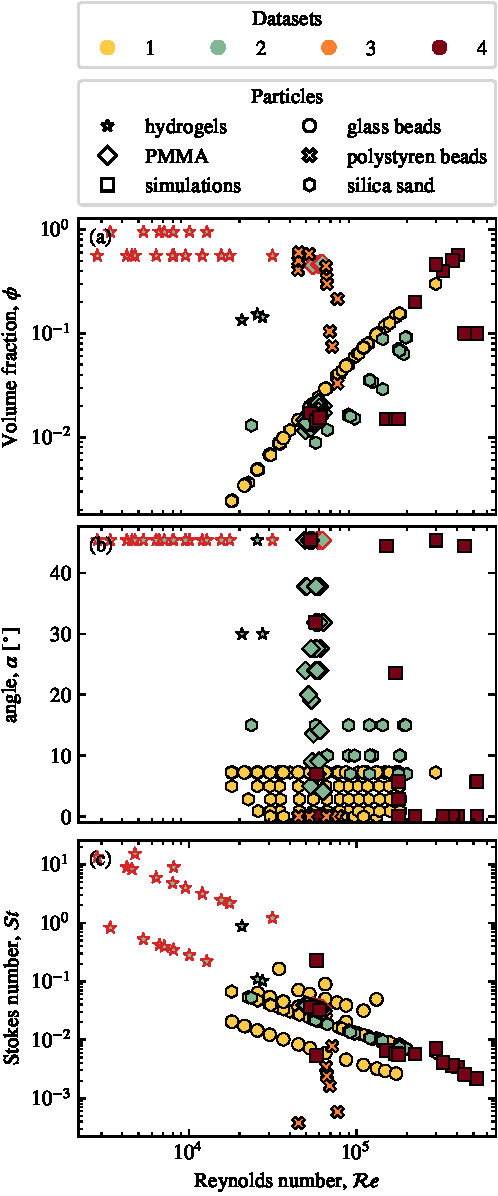
\includegraphics{figure2.pdf}
	\caption{\textbf{Explored parameter space.} Each symbol corresponds to a single experimental run. Red-edged symbols correspond to experimental runs starting with deposited particles inside the lock.}
	\label{fig:fig2}
\end{figure}
%%%%%%%%%%

Following section~\ref{sec:intro} and \ref{sec:methods}, the relevant length, velocity and time scales for the propagation of a lock-release gravity current are the lock-length $L_{0}$, the buoyancy velocity $U_{0}=\sqrt{g' H_0 \cos\alpha}$ and $t_{0} = L_{0}/U_{0}$, respectively.
%
Note that here, the reduced gravity $g' = g (\rho_{\text{m}}-\rho_{\text{a}})/\rho_{\text{a}}$ is different from $\tilde{g}$ defined in \eqref{eq:solUc} in order to include the dependence of the front velocity on the density ratio $\rho_{\text{m}}/\rho_{\text{a}}$ in the definition of $U_{0}$ (see \eqref{eq:Froude_Huppert1980} in section~\ref{sec:intro_lockrelease}), and in the resulting dimensionless quantities. As such, the velocity scale $U_0$ corresponds to an idealized transfer of initial potential energy to kinetic energy along the slope, i.e. a collapse of the initial column.

In addition to the particle volume fraction $\phi$ and bottom slope $\alpha$, we define the following control dimensionless parameters
\begin{equation}
	\displaystyle a =\frac{H_0}{L_0},
\end{equation}
\begin{equation}
	\displaystyle \mathcal{A}t = \frac{\rho_{\text{m}}-\rho_{\text{a}}}{\rho_{\text{a}}},
\end{equation}
\begin{equation}
	\displaystyle \mathcal{R}e = \frac{U_0 H_0\rho_{\text m}}{\eta_{\text f}},
\end{equation}
\begin{equation}
	\displaystyle \mathcal{S}t = \frac{L_{0} V_{\text s}}{H_{0} U_0},
\end{equation}
%
with $\eta_{{\text f}}$ is the interstitial fluid viscosity. Note that $\mathcal{S}t=S/a$ with $S$ is the dimensionless settling velocity as defined in section \ref{sec:intro_PLGC}. As an estimation of $V_{\text s}$, we neglect possible turbulent drag effects and particle-particle interactions in the settling process, leading to the Stokes settling velocity $V_{\text s} = d^{2}(\rho_{\text{p}} - \rho_{\text{f}})g/(18\eta_{{\text f}})$.
%
In the following, we assume that the particle influence on the current dynamics can be quantified by $\phi$ and $\mathcal{S}t$, and discard other dimensionless parameters involving grain properties (e.g. $H_{0}/d$, $\rho_{\text p}/\rho_{\text{f}}$).
%
Likewise, excess buoyancy effects will be taken into account through $U_{0}$, as $\mathcal{A}t$ is mostly used to quantify non-Boussinesq effects, which can be neglected here as for the large majority of the experiments and simulations, $\mathcal{A}t < 0.2$.

The dimensionless control parameters $\phi$, $\alpha$, $\mathcal{S}t$ and $\mathcal{R}e$, used in the 3 experimental datasets and in the numerical dataset, are shown in figure~\ref{fig:fig2}. Here, $\phi$, $\alpha$ and $\mathcal{S}t$ are reported against $\mathcal{R}e$. It is shown that they roughly cover the range $\phi \in [0.001, 0.5]$ (see description of dataset 2 in section~\ref{sec:datasets} for experiments with $\phi > 0.5$), $\alpha \in [0,45]^\circ$, $\mathcal{S}t \in [3{\times}10^{-3}, 10^{1}]$ and $\mathcal{R}e \in [10^3, 10^6]$. To finish with, the aspect ratio $a=H_0/L_0$ is varied in the range $[0.5, 5]$, but not systematically. As its influence can not be systematically quantified, this will rather be qualitatively discussed in section~\ref{sec:conclusion}.

\subsection{Macroscopic description of the current dynamics}

%%%%%%%%%%%%%%%%%%%% Figure 3
\begin{figure*}[ht]
	\centering
	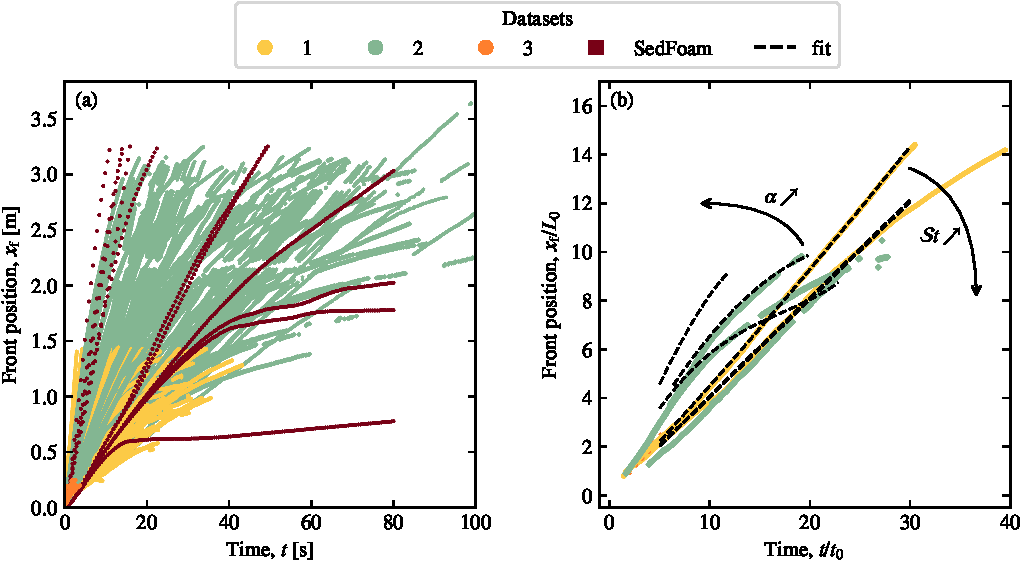
\includegraphics{figure3.pdf}
	\caption{(a) Current front position as a function of time for all experimental runs (b) Selected runs plotted in non-dimensional coordinates.}
	\label{fig:fig3}
\end{figure*}
%%%%%%%%%%%%%%%%%%%%

The current dynamics is characterized by the evolution of several dimensionless variables. Here, as stated in section~\ref{sec:intro}, we aim at giving a macroscopic description of the initial current dynamics across ranges of several parameters spanning multiple orders of magnitude. The wide diversity of experiments and simulations results in a large variety of currents which does not allow for an exhaustive description of their individual dynamics. We rather choose to focus on a single variable, the front position $x_{\text{f}}$, which has been shown in the literature to be a good proxy to describe the current dynamics~\citep[e.g.][]{bonnecaze1993particle, Chowdhury2011, Adduce2012}.

Figure~\ref{fig:fig3}(a) shows the front position of all experiments and simulations in dimensional coordinates, and figure~\ref{fig:fig3}(b) exhibits some selected runs in dimensionless coordinates. After a short transient acceleration phase, most currents exhibit at first a constant velocity phase, which corresponds to the so-called \emph{slumping} regime discussed in section \ref{sec:intro}. Afterwards, the velocity becomes time-dependent, often decreasing, due to one or multiple of the attenuation processes described in section~\ref{sec:intro}.
%
Qualitatively, it can be seen that increasing the bottom slope increases the slumping velocity while increasing the Stokes number shortens the duration of the constant-velocity phase (see fig~\ref{fig:fig3}).

In order to properly quantify the slumping regime, i.e. the associated front velocity and duration, it is necessary to prescribe the relevant attenuation process leading to the regime transition. Yet, this is a priori unknown given the variety of involved processes in the wide range of PLGCs parameters used here. We thus propose to overcome this issue by fitting experimental and numerical front evolution by a second-order temporal expansion of the front position $x_{\text f}(t)$ as
\begin{equation}
	\label{eq:fit_eq}
	\frac{x_{\text f}}{L_{0}} = \frac{x_{i}}{L_0} + \mathcal{F}r \left[\frac{t}{t_{0}} - \frac{1}{\tau} \left(\frac{t}{t_{0}}\right)^{2}\right],
\end{equation}
where $\mathcal{F}r = U_{\text{c}}/U_{0}$ corresponds to the dimensionless current velocity during the slumping regime and $\tau$ to a dimensionless attenuation time scale related to $X_{\text{t}}$ as
\begin{equation}
	\label{eq:link_Xt_tau}
	\frac{X_{\text{t}}}{L_{0}} \propto \tau\mathcal{F}r.
\end{equation}
Note that the previous expansion \eqref{eq:fit_eq} assumes a constant velocity and constant deceleration trend of the front evolution. The latter is relevant to extract the time scale of existence of the slumping regime, i.e. the linear component, as long as its dynamics has only weakly deviated from such linear evolution. It is thus required to consider such a solution only during a brief time scale beyond the linear slumping regime.
%as defined here, $\mathcal{F}r$ is not a control parameter, but a dimensionless variable characteristic of the initial current dynamics (The Froude number which would be defined as a control parameter for a lock-release configuration would be $\mathcal{F}r \equiv U_{0}/U_{0} = 1$, and is thus not relevant to describe the flow dynamics).

In the following, we fit all front propagation curves (except for dataset 3) with \eqref{eq:fit_eq} between $t/t_{0} = 5$, to avoid the initial transient phase, and $t/t_{0} = 30$, the transition time from the slumping to the inertial regime~\citep[similar to $X_{\text{t}}/L_{0}\approx 10$ as mentioned in section \ref{sec:intro_lockrelease}; see also e.g.][]{Rottman1983, Sher2015, Ottolenghi2016}. Note that $x_{i}$ is kept constant equal to 0 for datasets 1 and 2, but had to be left free to adjust for the SedFoam simulations. This is probably due to the influence of the initial condition. In most of the experiments, due to the stirring, the initial condition exhibits velocity fluctuations as well as concentration fluctuations which might influence the early current behaviour. In the 2D RANS two-fluid simulations using sedFOAM, the velocities are zero and the concentration is homogeneous, both without any fluctuations. For runs with strong attenuation ($\tau < 10^{2}$), we add a quartic term to \eqref{eq:fit_eq} to improve the fit quality and obtain a better estimation of $\mathcal{F}r$ and $\tau$. We checked that our results do not depend on the presence of this quartic term and that the linear and quadratic ones remain much larger. Finally, for dataset 3, the time resolution and the experiment duration do not allow for inferring the quadratic term. Therefore, we simply fit the whole available points with a linear function.

\section{Results}
\label{sec:results}

\subsection{Influence of the bottom slope, $\alpha$}
\label{sec:influence_slope}

In this section, we focus on the influence of the bottom slope $\alpha$ on the current dynamics. Hence, figure~\ref{fig:fig4} shows the dimensionless front velocity $\mathcal{F}r$ as a function of $\alpha$ for the entire set of experiments.

Despite the scatter in our experimental points, $\mathcal{F}r$ clearly exhibits an increasing trend with $\alpha$. Note however that the exact shape of this trend remains unclear, especially close to $\alpha=0^\circ$, where the various datasets may suggest slightly different trends. Note also the large scatter at $\alpha=45^\circ$, mostly related to experimental data points with $\phi > 0.45$ (transparent markers) and a settled initial condition (red-edged markers, see description of dataset 2 in section~\ref{sec:datasets}).
%
Such evolution of $\mathcal{F}r$ with $\alpha$ has only been reported few studies of homogeneous saline currents with either experiments on a smaller range of slopes $\alpha$ \citep{Maxworthy2007} or numerical simulations for small aspect-ratio $a = 0.1$ \citet{Birman2007}. This suggests a mechanism independent of the properties of the dense fluid, either saline or particle-laden. Interestingly, our data exhibits a much larger dependency of $\mathcal{F}r$ on $\alpha$ than reported in these simulations at small $a$. This difference is thus probably due to a significant difference in the lock aspect-ratio, which has been shown to significantly affect $\mathcal{F}r$ for $\alpha=0$ (see \citet{Bonometti2011} for instance), rather than from the presence of particles, as further discussed in sections~\ref{sec:influence_stokes} and~\ref{sec:influence_phi}.

It shall be noted that this dependency of the slumping velocity on the bottom slope exists despite the slumping equilibrium being unmodified by the presence of a slope-induced acceleration (see section~\ref{sec:intro} for details). As suggested in \citet{Gadal2023}, the latter acceleration may instead affect the complicated dynamics of the early transient acceleration phase, involving strong vertical motions and significant interfacial friction~\citep{Cantero2007}.
%
One can write an energetic balance between the initial state and the end of this early acceleration phase \citep{Gadal2023}
\begin{equation}
	\label{eq:energetic_balance}
	\left[\frac{1}{2}\rho_{0}u_{\text c}^{2} - B \Delta\rho g \sin\alpha L\right] - A \Delta\rho g \cos\alpha h_{0} =  - \frac{1}{2}c_{\text d}\rho_{0}u_{\text c}^{2} \frac{L}{h_{0}},
\end{equation}
where $A$, $B$ and $c_{\text d}$ are scaling constants, and $L$ accounts for the along slope distance over which the current moves during this phase. \citet{Cantero2007} found it to be independent of the lock aspect ratio or initial buoyancy, $L = 0.3 h_{0}$. Hence, we use here $L = D h_{0}$ with $D$ constant, which results in
\begin{equation}
	\label{eq:Fr_th}
	\mathcal{F}r = \frac{U_{\text c}}{U_0} = \frac{Fr_0}{\sqrt{1 + C_{\text D}}} \sqrt{1 + \frac{\tan\alpha}{S}},
\end{equation}
where $Fr_0$, $C_{\text D}$ and $S$ are new constants depending on $A$, $B$, $c_{\text d}$ and $D$. As shown in Fig.~\ref{fig:fig4}, this simple model is able to reproduce the observed variation of the dimensionless velocity in the bottom slope in the range [$5^\circ$, $35^\circ$].
%
For $\alpha < 5^\circ$, experimental data points are significantly scattered, and \eqref{eq:Fr_th} almost systematically overpredicts the $\mathcal{F}r$ values. A plausible explanation for this discrepancy could be the difference in the width-to-depth ratio of the flumes (and associated wall dissipation) and in aspect ratios of the lock, which are not addressed in the energetic balance leading to \eqref{eq:Fr_th}.
%
For $\alpha > 35^\circ$, the measured dimensionless velocities ($\mathcal{F}r$) slowly stand above equation (\ref{eq:Fr_th}) curve. In this region of large slope angles, it is likely that the equilibrium between the forces becomes a lot more in favour of the so-called slope effect than the pressure gradient. Consequently, the scaling constants may have to be adapted to this major change in the influence of the forces.

\begin{figure*}[ht]
	\centering
	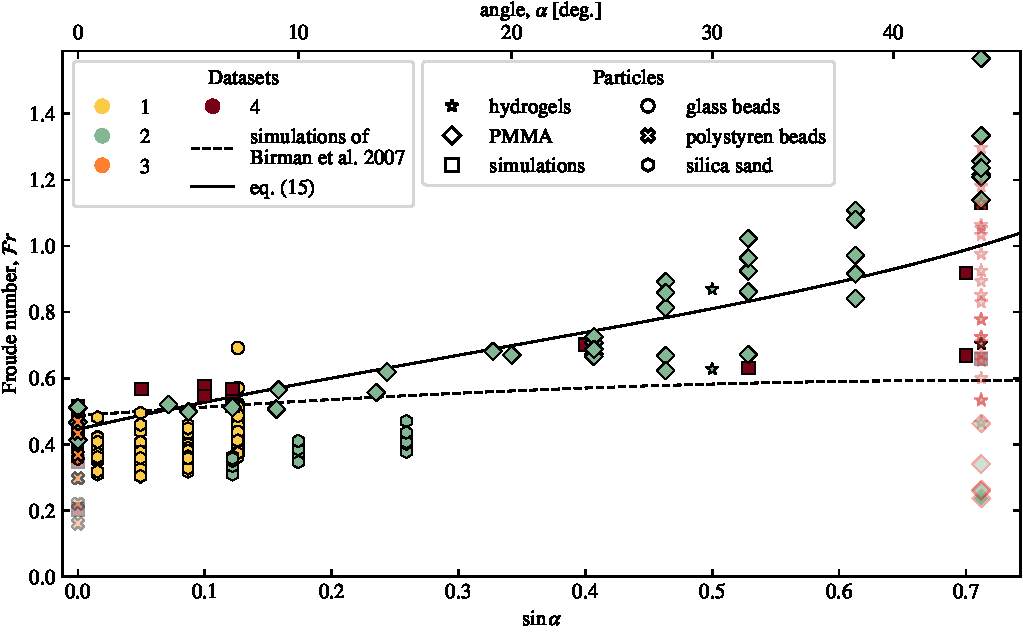
\includegraphics{figure4.pdf}
	\caption{\textbf{Influence of the bottom slope} on the current Froude number. Plain symbols correspond to $\phi < 0.45$, while transparent symbols are for $\phi \geq 0.45$ (see section~\ref{sec:influence_phi} for details on the influence of $\phi$). The black plain line indicates the prediction of \eqref{eq:Fr_th} for $Fr_{0} = 0.5$, $C_{\text D} = 0.4$ and $S = 0.25$. The black dashed line indicates the fit to the data from the numerical simulation of \citet{Birman2007} for saline homogeneous gravity currents.}
	\label{fig:fig4}
\end{figure*}

\subsection{Influence of the Stokes number, $\mathcal{S}t$}
\label{sec:influence_stokes}

\begin{figure*}[ht]
	\centering
	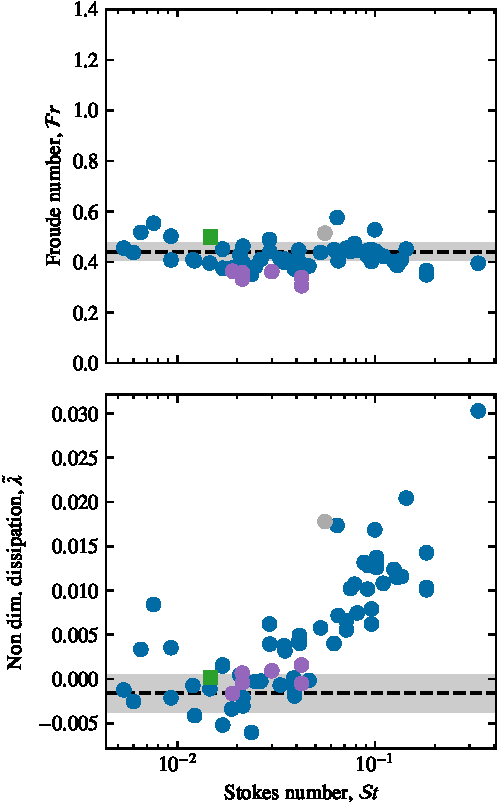
\includegraphics{figure5.pdf}
	\caption{\textbf{Influence of particle settling.} Current Froude number $\mathcal{F}r$ and attenuation $1/\tau$ as a function of the ratio between the Stokes number and the lock aspect-ratio, for different ranges of bottom slopes. Plain symbols correspond to $\phi < 0.45$, while transparent symbols are for $\phi \geq 0.45$ (see section~\ref{sec:influence_phi} for details on the influence of $\phi$). Dotted lines mark either the average of points with $\phi < 0.45$ (a, c, e, g) or the 0 baseline (b, d, f, h). On (e, f), the dashed line indicates the average value for homogeneous saline currents ($St \equiv 0$) of dataset 1. On (b, d, f, h), the black line is $1/\tau = 0.27 (St - 0.015)$.}
	\label{fig:fig5}
\end{figure*}

In this section, we focus on the influence of settling on the current dynamics. The influence of the Stokes number $\mathcal{S}t$ on the dimensionless front velocity $\mathcal{F}r$ and attenuation $\tau$ is presented in figure~\ref{fig:fig5} for different bottom slopes $\alpha$.

At the first order, the dimensionless front velocity does not depend on $\mathcal{S}t$ (see figure~\ref{fig:fig5}a, c, e). However, this is not the case for the attenuation time scale $\tau$. For $\alpha \approx 7^\circ$, the attenuation ($1/\tau$) is constant below a threshold $St_{\text c} \simeq 10^{-2}$, but increases rather linearly above this value (see the black line in figure~\ref{fig:fig5}(d), note the semi-log x-scale).

These two regimes can be understood as follows. First, assuming that the current decelerates due to its transition from the slumping regime towards the so-called \emph{inertial} regime, combining \eqref{eq:Xt_inertial} and \eqref{eq:link_Xt_tau} results in $\tau \sim cste$. Then, if the current decelerates due to a settling-induced loss of buoyancy, combining \eqref{eq:Xt_settling} and \eqref{eq:link_Xt_tau} results in
%
\begin{equation}
	\frac{1}{\tau} \sim \mathcal{S}t.
\end{equation}
%
This corresponds well to the observed trend in figure~\ref{fig:fig5}(d), hence confirming that above $St_{\text c} \simeq 10^{-2}$, particle settling controls the end of the slumping regime. Similar results can also be extrapolated for $\alpha = 0^\circ$ and $\alpha = 15^\circ$, although additional points are required to assess the dependence of the transitional threshold and of the slope of the linear increase with $\phi$ or $\alpha$.

For larger slopes, our experiments do not allow us to discriminate the influence of the Stokes number (see figure~\ref{fig:fig5}(g,h)). From further exploring of these regimes might arise singular effects as, at large slopes, a significant component of the settling occurs along the slope. It might therefore contribute to increasing the current inertia, or at least to decreasing the expected attenuation.

\subsection{Influence of volume fraction, $\phi$}
\label{sec:influence_phi}

\begin{figure}
	\centering
	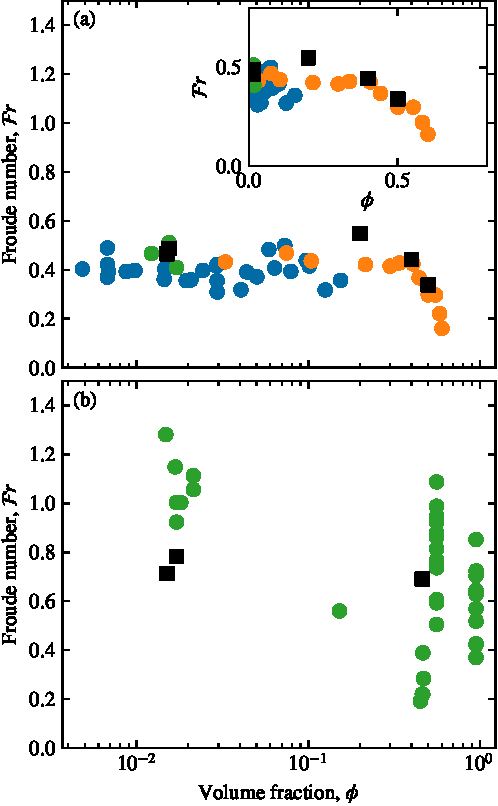
\includegraphics{figure6.pdf}
	\caption{\textbf{Influence of particle volume fraction.} Current Froude number as a function of the initial particle volume fraction for (a) $\alpha \approx 0^\circ$, and (b) $\alpha \approx 45^\circ$. The inset in (a) shows the plot in linear scale. The black line indicates the prediction of \eqref{eq:Fr_th_eta} for $Fr_{0} = 0.5$, $C_{\text D} = 0.4$, $S = 0.25$ and $Re_{\text c} = 500$.}
	\label{fig:fig6}
\end{figure}

In this section, we focus on the influence of the particle volume fraction $\phi$ on the current dynamics. Hence, figure~\ref{fig:fig6} shows the dimensionless front velocity $\mathcal{F}r$ as a function of $\phi$ for $\alpha=0^\circ$ and $\alpha=45^\circ$.

For $\alpha=0^\circ$, figure~\ref{fig:fig6}(a) shows that $\mathcal{F}r$ is independent of $\phi$ up to a critical value $\phi_{c} \simeq 0.45$, above which the Froude number abruptly decreases. This results from the large increase in effective viscosity induced by the presence of particles~\citep{stickel2005fluid}, which probably enhances dissipation at the bottom and on the sidewalls. Furthermore, this decrease in Froude number is associated with a reduction of the height of the current in the presence of a strong mass gradient near the front, as noted by \citet{Schneider2023}.


The energetic balance presented in section~\ref{sec:influence_slope} can be adapted to include viscous dissipation effects, by replacing the constant $c_{\text d}$ in \eqref{eq:energetic_balance} by:
\begin{equation}
	c_{\text d}\left(1 + \frac{E}{\mathcal{R}e}\frac{U_0}{U_{\text c}}\frac{\eta_{\text eff}}{\eta_{\text f}} \right),
\end{equation}
where $E$ is a new scaling constant, and $\eta_{\text eff}$ is the effective suspension viscosity accounting for the presence of particles. This results in
\begin{equation}
	\label{eq:Fr_th_eta}
	\begin{split}
		\mathcal{F}r & =  \frac{1}{1 + C_{\text D}} \left[-\frac{Re_{\text c}}{\mathcal{R}e}\frac{\eta_{\text eff}}{\eta_{\text f}} \right. \\
		&\left. +\sqrt{\left(\frac{Re_{\text c}}{\mathcal{R}e}\frac{\eta_{\text eff}}{\eta_{\text f}} \right)^{2} + Fr_0^{2} \left(1 + \left[1 + C_{\text D}\right]\frac{\tan\alpha}{S} \right)}  \right],
	\end{split}
\end{equation}
where $Re_{\text c}$ is a new constant. The effect of the particles on the effective viscosity is based on the correlation proposed by \citet{krieger1959mechanism} and validated in many configurations:
\begin{equation}
	\label{eq:Krieger}
	\frac{\eta_{\text eff}}{\eta_{\text f}} = \left(1 - \frac{\phi}{\phi_{\text m}}\right)^{-(5/2)\phi_{\text m}},
\end{equation}
where $\phi_{\text m} = 0.585$ is the maximum volume fraction~\citep{boyer2011unifying}.
%
As shown in figure~\ref{fig:fig6}(a), the combination of equations \eqref{eq:Fr_th_eta} and \eqref{eq:Krieger} can reproduce quantitatively the observed influence of $\phi$ on the dimensionless velocity for $\alpha=0^\circ$. This agreement does not depend on the choice of the viscosity model, and using other available rheological models from the literature~\citep{stickel2005fluid, boyer2011unifying} leads to the same conclusions.

For $\alpha=45^\circ$, a decreasing trend of the dimensionless front velocity is also observed despite the dispersion of experimental points. However, the shape of this trend is less clear, especially because data at large $\phi$ correspond to a different initial condition (red-edged markers, see description of dataset 2 in section~\ref{sec:datasets}), which makes the interpretation difficult. The combination of \eqref{eq:Fr_th_eta} and \eqref{eq:Krieger} is shown for completeness.

\section{Conclusion and perspectives}
\label{sec:conclusion}

\begin{figure*}[ht]
	\centering
	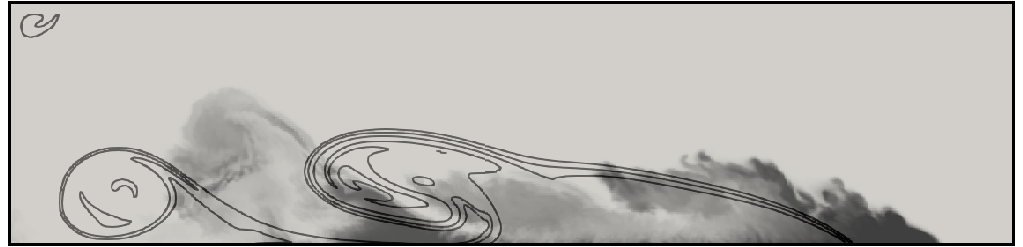
\includegraphics{figures/figure7.pdf}
	\caption{Comparison between 2D (lines) and 3D (grey scale) two-fluids numerical simulation at $t = 15~\textrm{s}$ ($t/t_{0} = 45$) for $\alpha = 45^\circ$, $\phi = 0.1$ and $St = 2{\times}10^{-2}$.}
	\label{fig:fig7}
\end{figure*}

In this chapter, we summarize the effect of various dimensionless parameters on the early propagation of finite-volume turbidity currents. Hence, by using data from multiple experimental devices and from two-fluid numerical simulations, we explore a wide range of $\phi$, $\alpha$, $\mathcal{S}t$ and $\mathcal{R}e$.
%
By reducing the early dynamics to a constant-velocity propagation at a dimensionless velocity $\mathcal{F}r$ during a dimensionless characteristic time $\tau$ (see~\eqref{eq:fit_eq} for additional details), we show that:
\begin{itemize}
	\item $\mathcal{F}r$ is independent of $\mathcal{S}t$, but increases with $\alpha$ and drastically decreases with $\phi$ above a critical value $\phi_{\text c} \approx 0.45$. These variations are well explained by a simple energy balance during the early transient acceleration phase occurring before the slumping regime for which the front evolves at constant velocity. This early stage dynamics is associated with a non-conservative and slope-dependent transfer of the initial potential energy towards the along-slope kinetic energy (see \eqref{eq:Fr_th}, \eqref{eq:Fr_th_eta}). The role of the particles in the dissipation is captured by considering an effective suspension viscosity model (\eqref{eq:Fr_th_eta}).

	\item $1/\tau$ depends on $\mathcal{S}t$ above a transition value $St_{\text c} \approx 10^{-2}$. Below $St_{\text c}$, the currents are then similar to a gravity current induced by a saline dense fluid, while above $St_{\text c}$, dissipation $1/\tau$ increases as $1/\tau \sim \mathcal{S}t$, or equivalently the duration of the slumping regime decreases as $\tau \sim \mathcal{S}t^{-1}$.
\end{itemize}
Although probably hidden by the first-order dependency (velocity) of the dynamics on these parameters, note that we also expect $\tau$ to depend on $\alpha$ and $\phi$.
%
Importantly, all these variations can also be quantitatively reproduced by the 2D vertical numerical simulations using a two-fluid model. This validates the use of continuous approaches over looking at the grain scale dynamics to understand and model these parts of the current dynamics.

% \begin{itemize}
%     \item Rationalize/Compare PLGCs dynamics using multiple devices
%     \item Si on ecrit vfront = \mathcal{F}r (1-1/tau t2), \mathcal{F}r (alpha,phi) et \mathcal{F}r ne depend pas de \mathcal{S}t. attenuation, tau (alpha, phi, \mathcal{S}t) on a montre la dependece en (\mathcal{S}t) et celle en alpha, phi car domine par l ordre 1.
%     \item Numerique diphasique EUler-Euler 2D, permet de retrouver ces tendances. Donc l echelle du grain n est pas primordiale pour comprendre tout ca.
% \end{itemize}

Altogether, the influence of $\phi$, $\mathcal{S}t$, $\alpha$ on the slumping dynamics of PLGCs characterised in the present study, highlights the importance of a better understanding of the early stage transfer of initial potential energy towards the along-slope kinetic energy. To predict the longtime scale evolution of PLGCs, the knowledge and the characterisation of their early-stage dynamics remain fundamental to prescribe an initial input for large-scale modelling.

However, details of the current shape and related mixing remain unclear. In particular, even even if the front velocity is well captured by the 2D simulations, they poorly capture the current shapes, as shown in figures~\ref{fig:fig1} and~\ref{fig:fig7}. This would require 3D simulations to properly capture the turbulent mixing at the current interface. For validation, advanced experimental metrologies are thus required to extract accurate measurements of the turbulent mixing at the interface and responsible for ambient entrainment in the current. These should be an important focus for future work.
%
Moreover, we also found that the choice in kinetic theory closures for the particle phases in the simulations can modify the measured velocities up to $30~\%$ (especially at larger slopes), which emphasizes the role of particle-particle interactions in the macroscopic dynamics of PLGCs. These are particularly important in zones of large volume fractions and are therefore key to quantifying the ability of a current to erode a loose sediment bottom or the dynamics of currents originating from deposited sediment. Both are common situations in natural flows and require the focus of future works.


%\begin{itemize}
%   \item Details of the current shape and associated mixing remains unclear
%  \item Then 3D numerical simulations are required, as 2D pourly capture the shape.
%\end{itemize}

% \julien{
% \begin{itemize}
%     \item Influence of kinetic theory closures suggests that the particle-particle interactions play a role in the dynamics of the PLGC.
%     \item 3D effects matter on the turbulent mixing at the current interface (add a figure with 2 snapshots)
%     \item Influence of the initial condition in the numerical simulations: noise on volume fraction, velocities, ... Relevant for 2D RANS simulations? 
% \end{itemize}
% }

% \cyril{
% \begin{itemize}
%     \item Influence of $a = H_{0}/L_{0}$ ? (add a figure $Fr = f(a)$ for $\alpha = 0$, $\alpha = 7$ ?)
%     \item Influence of $H_{0}/d$ for setting/maintaining particles in suspension (`pore pressure')? Relevant for experiments with initial deposited experiments and for strong settling?
%     \item Part of $V_{s}\sin\alpha$ that increases current inertia ?
% \end{itemize}
% }

% \begin{itemize}
%     \item Future works need to focus on the link between this dynamics and the ability to erode the bottom, as observed in natural flow.
% \end{itemize}

\subsection*{Data availability}

Data and processing scripts are available at [public repository DOI] (will be completed upon publication).

\subsection*{Acknowledgment}
We thank Jean-Dominique Barron (IMFT) and Sébastien Cazin (IMFT) for their support in carrying out the experiments on setup-up 1.
%
Sylvain Dauge is acknowledged for the full design of setup 2. Hervé Bellot and Brivaël Collin are thanked for their experimental support.
%
We also acknowledge Hugo Divel for his contribution to the preliminary lock-release simulations using SedFoam.
%
Finally, we would like to acknowledge the contributors of the open-source numerical Python libraries, including Matplotlib \citep{Hunter2007}, NumPy \citep{Harris2020} and SciPy \citep{Virtanen2020}, which provide an incredibly efficient ecosystem allowing scientific research in Python.

\subsection*{Fundings}
We acknowledge financial support from the French National Research Agency Grants, ANR-19-CE30-0041/PALAGRAM.

\bibliographystyle{apalike}
\bibliography{biblio}

\end{document}